% Over the last three decades, researchers have proposed approximately 400 different activation functions \cite{Kunc2024}, suggesting a vast landscape of possibilities for neural network optimization. Historically, models such as those based on the transformer architecture, introduced in initial transformer paper \cite{Vaswani2017}, predominantly utilized Rectified Linear Unit (ReLU). However, the landscape began shifting when other activation functions started being considered.

% A pivotal moment in the evolution of activation functions in language models was marked by the introducction of the Gaussian Error Linear Unit (GELU)\cite{Lee2023}. GELU has become the popular choice for language models and it's also the default activation function RoBERTa and GPT-Neo, implemented by Hugging Face which are the ones I will be using as my baseline. This function's popularity underscores its perceived utility over traditional functions like ReLU in specific contexts, particularly in models with parameters on the scale of hundreds of millions.

% Yet, as already mentioned, a significant research gap persists in comparison of activation functions, particularly on models smaller than 100m parameters. This gap could be explained by findings from another paper, which suggests that the impact of activation functions diminishes as the model size increases, evident in models with over a billion parameters \cite{Mirzadeh2023}. This also explains the initial move away from ReLU, since all the research on alternatives was done on models with the size of approximately 100 million parameters.

% Given these insights, this research will explore the impact of various activation functions on smaller-scale language models with around 10 million parameters. The hypothesis posits that at smaller scales, the choice of activation function is crucial, potentially leading to significant performance variations.

% Further, this research will delve into an area of adaptive activation functions. It has been shown that adaptive activation functions outperform static ones in text-to-text machine translation \cite{Rajanand}, but there seems to be a lack of further research into adaptive function in language models, likely due to an expected tradeoff between additional trainable parameters and impact on performance. Additionally, recent developments in KAN: Kolmogorov-Arnold Networks \cite{Liu2024} suggest a shift towards using activation functions on edges instead of nodes, but due to its recency, it has yet to be tested on a language model. This research will also experiment with this concept and apply it to language modeling to assess its efficacy at smaller scales.

% This paper will structure its discussion starting with a review of historical and current activation functions, followed by methodology, experimental setup, results, and conclusions. By addressing these facets, the study aims to illuminate how different activation functions can enhance or compromise the performance of scaled-down language models, ultimately contributing to the optimization of neural network design.
\clearpage
\section{Background and related work}
% ** Quick explanation of activation functions ** NOTE: Fix up this paragraph
% - Activation functions are used to introduce non-linearity to neural networks
% - they are on nodes 

% ** Timeline of activations in LLMs **
% - "Attention is all you need" \cite{Vaswani2017} just used the state of the art activation function at the time, ReLU
% - No siginficant improvements till GELU \cite{Lee2023} was introduced which soon became the default activation function in LLMs
% - Development continues new alternatives presented such as GeGLU \cite{Shazeer2020}

% ** The gap **
% - sigmoind -> (models bigger) -> ReLU -> (models bigger) -> GELU -> (models bigger) -> back to relu
% - as mentioned gap of comprehesive comparison of activation functions especially in smaller models
% - the gap can be explained by findings from a recent paper that suggests move back to ReLU as the impact of activation functions diminishes as the model size increases \cite{Mirzadeh2023}
% ADAPTIVE FUNCTIONS GAP
% - another interesting gap is the lac of research of adaptive activation functions in LLMs, only one paper found \cite{Rajanand} which found ... (insert here)
% - very recent development addressing performace of smaller models is KAN: Kolmogorov-Arnold Networks \cite{Liu2024} which suggests a shift towards using activation functions on edges instead of nodes

% ** KAN bacground and gap **
% - KAN is a new type of neural network that uses activation functions on edges instead of nodes
% - It has been shown to outperform traditional neural networks in some tasks \cite{Liu2024}
% - It seems to be mostly suited for scientific applications such as solving partical differential equations \cite{Liu2024}
% - but at the time of my research no tests on LLMs have been done yet
% - the main benefit is optimizing activation on each edge insted of node, using something called splines 
% - the main drawback is the increased number of trainable parameters

% NOTE: Fix Lee2023 citation for GELU
Activation functions are used to introduce non-linearity into neural networks, allowing them to model complex relationships in the data. They are applied to the nodes of the network and are essential for enabling the network to learn and perform a wide range of tasks, beyond what linear models can achieve.

The famous paper "Attention is All You Need" \cite{Vaswani2017} used the state-of-the-art activation function at the time, ReLU. Since then, no significant improvements were made until the introduction of GELU, which quickly became the default activation function in most of the state-of-the-art LLMs \cite{Lee2023}. The popularity of GELU stems from its ability to enhance model performance without introducing an efficiency overhead. Despite these advancements, continuous innovation leads to alternatives like GeGLU, noted for its effectiveness \cite{Shazeer2020}, also used in last year's winner of the BabyLM challenge \cite{Samuel2023}. However, a recently published paper suggests a return to ReLU \cite{Mirzadeh2023}, adding further confusion to the search for the optimal activation function. Fortunately, it also provides some clues that guide further exploration and motivate this research.

The paper suggests that suggests that the impact of activation functions diminishes as the model size increases, evident in models with over a billion parameters \cite{Mirzadeh2023}. This also explains the initial move away from ReLU, since all the research on activation alternatives was done on models with the size of approximately 100 million parameters. Highlighting this finding further motivates the need to investigate activation functions in 10 million parameter models. The impact of activation functions is expected to be more significant in smaller models, and until now, decisions have been made with the trend of increasing model size in mind.

Furthermore, another gap appears in the research on activation functions with trainable parameters (adaptible activaition functions). The possible explanation for this could be the tradeoff between additional trainable parameters and performance. However, this was primarily studied in larger models. The only paper found on adaptive activation functions in LLMs is by Rajanand et al. \cite{Rajanand}, which found that adaptive activation functions outperform static ones in text-to-text machine translation [NOTE: add the exact numbers from the paper], a task closely related to language models. This suggests that adaptive activation functions could be beneficial for smaller models, but further research is needed to confirm this hypothesis. Given these insights, this research will explore the impact of various activation functions on smaller-scale language models with around 10 million parameters. Hypothesising that at smaller scales, the choice of activation function is crucial and having learnable parameters could be beneficial.

Kolmogorov-Arnold Networks (KAN) represent a recent development in neural network architecture, where activation functions are applied on edges instead of nodes \cite{Liu2024}. This approach has been shown to outperform traditional neural networks in some tasks, particularly in scientific applications such as solving partial differential equations. However, at the time of this literature review, it has yet to be tested on language models. The primary benefit of KAN is the optimization of activation on each edge using splines. A spline is a piecewise-defined polynomial function used in interpolation and approximation to create smooth curves through a set of points [ADD REFERENCE]. With a spline on each edge, each edge can have its own custom activation function, trained separately and uniquely shaped. In contrast, adaptive activation functions have the same shape but different gradients. Although this comes with the drawback of an increased number of trainable parameters. This research will experiment with applying KAN to language modeling to assess its efficacy at smaller scales, filling the gap in current literature.
\clearpage
\vspace*{\fill}
\begin{figure}[hb]
    \centering
    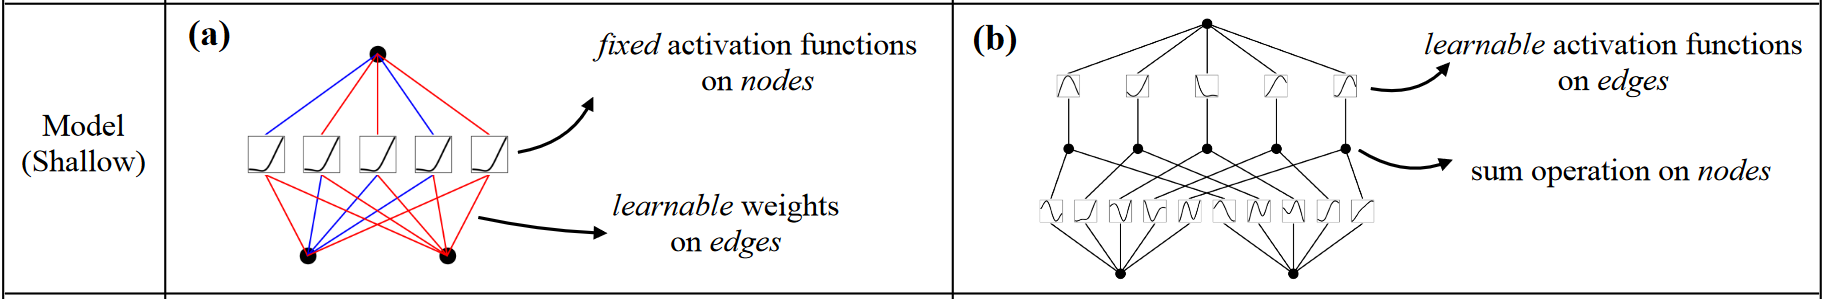
\includegraphics[width=\columnwidth * 2]{figures/kan-network.png}
    \caption{KAN vs MLP [3]}
    \label{fig:your-label}
\end{figure}
\vspace*{\fill}

\clearpage